\chapter{Dynamic Program}
\label{ch:dynprog}

We describe two algorithms that aim to decide Problem~\ref{prob:weak-udc-lobster} on a lobster instance of size $n$ in time linear in $n$. The \emph{dynamic program} is an implementation of the algorithm conceptualized in the literature~\cite{Bhore2021}, with a few refinements for practical performance. It solves Problem~\ref{prob:weak-udc-lobster} exactly, i.e. if the lobster admits a tri-grid x-monotone embedding, the dynamic program produces the correct decision as its output.

Dynamic programming is a technique whereby a problem is solved by dividing it into smaller sub-problems and combining their solutions.
A key feature of this approach is the reuse of solutions to sub-problems which emerge in different problem divisions.

\begin{figure}
    \centering
    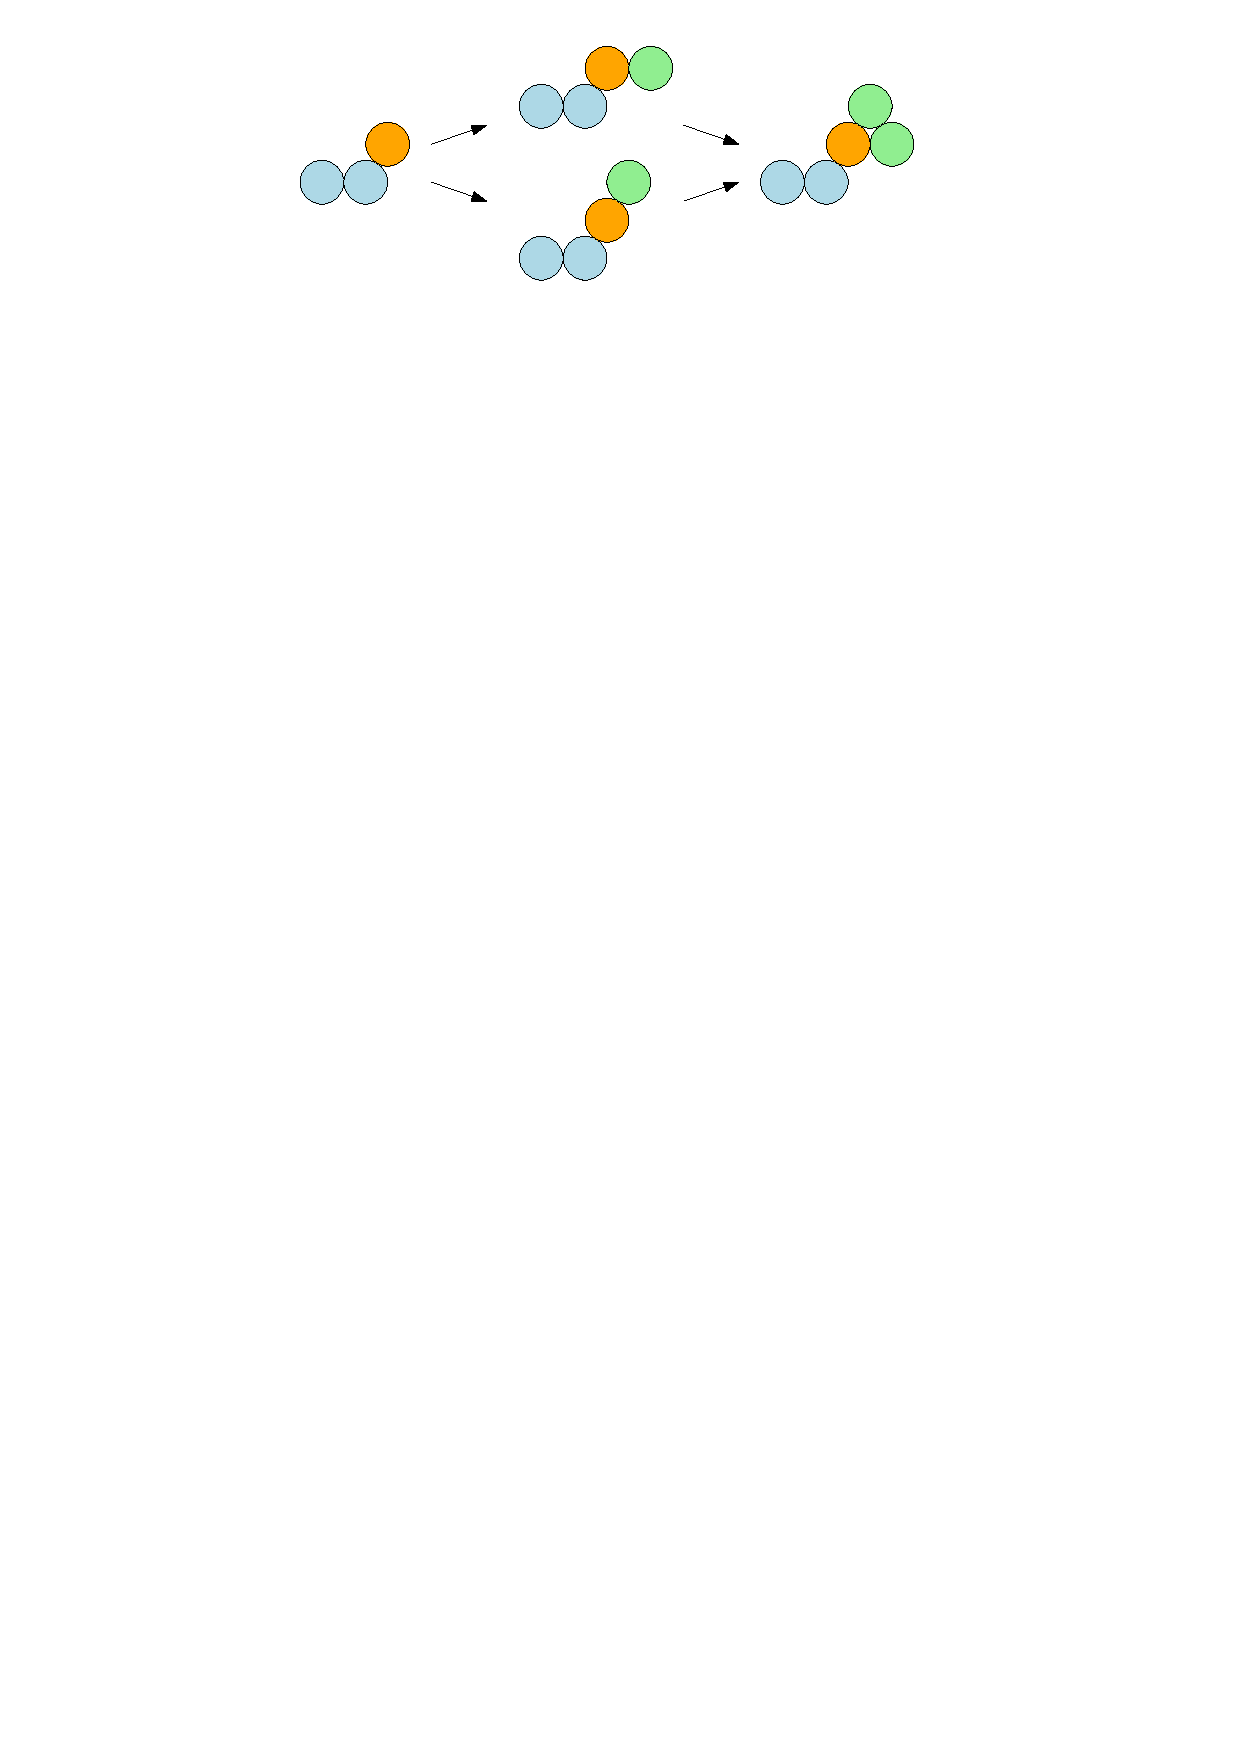
\includegraphics{graphics/ch4_reuse.pdf}
    \caption{Problem reuse in the dynamic program. The disk configurations represent some partial UDC representations of a lobster corresponding to partial problems. These result from decisions of the dynamic program during subdivision. A partial problem subdivides into several partial problems, among them the ones following the arrows.
    Note that the representation on the right side results from subdivision of different problems. The key to the efficiency of the dynamic programming approach is that we solve this problem at most once, even though we may encounter it from multiple predecessors. We can reuse its answer to answer both the sub-problems in the middle.
    In other words, we only remember one unique copy of the signature for the new partial problem.
    }
    \label{fig:ch4_reuse}
\end{figure}

\section{Problem Definition}
\label{section:ch4-probdef}
To apply the dynamic programming idea to problem~\ref{prob:weak-udc-lobster}, we must extend its definition to that of the \emph{partial recognition problem} which we introduce in this section.

Let $G = (V, E), V = \Spines \cup \Branches \cup \Leaves$ be a lobster. 

The \emph{embedding order} $\order$ for $G$ is a total order over $V$. It dictates the order in which the algorithm assigns coordinates to vertices in its exploration of the partial problem space. Starting from the initial problem, where no vertices are embedded, the minimum vertex under $\order$ gets the first assigned coordinate. The final coordinate assignment to the maximum vertex implies an affirmative answer to the original problem instance. 

An embedding order $\order$ is \emph{admissible} if it fulfills the following criteria.

\begin{itemize}
    \item $\order$ is a total order. It is reflexive, transitive and antisymmetric.
    \item $\order$ orders the spine.
    \begin{itemize}
        \item There exists a minimal $v_0 \in \Spines$ --- $\forall v \in V: v_0 \order v$ --- which is connected to $\leq 1$ other spines.
        \item Let $s_1, s_2, s_3 \in \Spines, s_1 \order s_2, s_1 \order s_3$\soeren{This seems off. Should this be $s_2 \order s_3$? And isn't that just Transitivity?}\peter{No, this is about the relationship between $\order$ and graph edges. The statement $s_2 \order s_3$ is the consequence of $s_1$ and $s_2$ being adjacent, not the premise.} and $(s_1, s_2) \in E$. Then $s_2 \order s_3$.
    \end{itemize}
    \item $\order$ groups branches together with their parent spine. Let $s_1, s_2 \in \Spines, b \in \Branches, s_1 = p(b)$ and $s_1 \order s_2$. Then $b \order s_2$.
    \item $\order$ groups subtrees together. Let $l \in \Leaves, b = p(l) \in \Branches, v \in V, (b, v) \not\in E$ and $b \order v$. Then $l \order v$.
    \item Parent vertices come first. Let $v_1, v_2 \in V$. If $v_1 = p(v_2)$, then $v_1 \order v_2$.
\end{itemize}

\begin{figure}
    \centering
    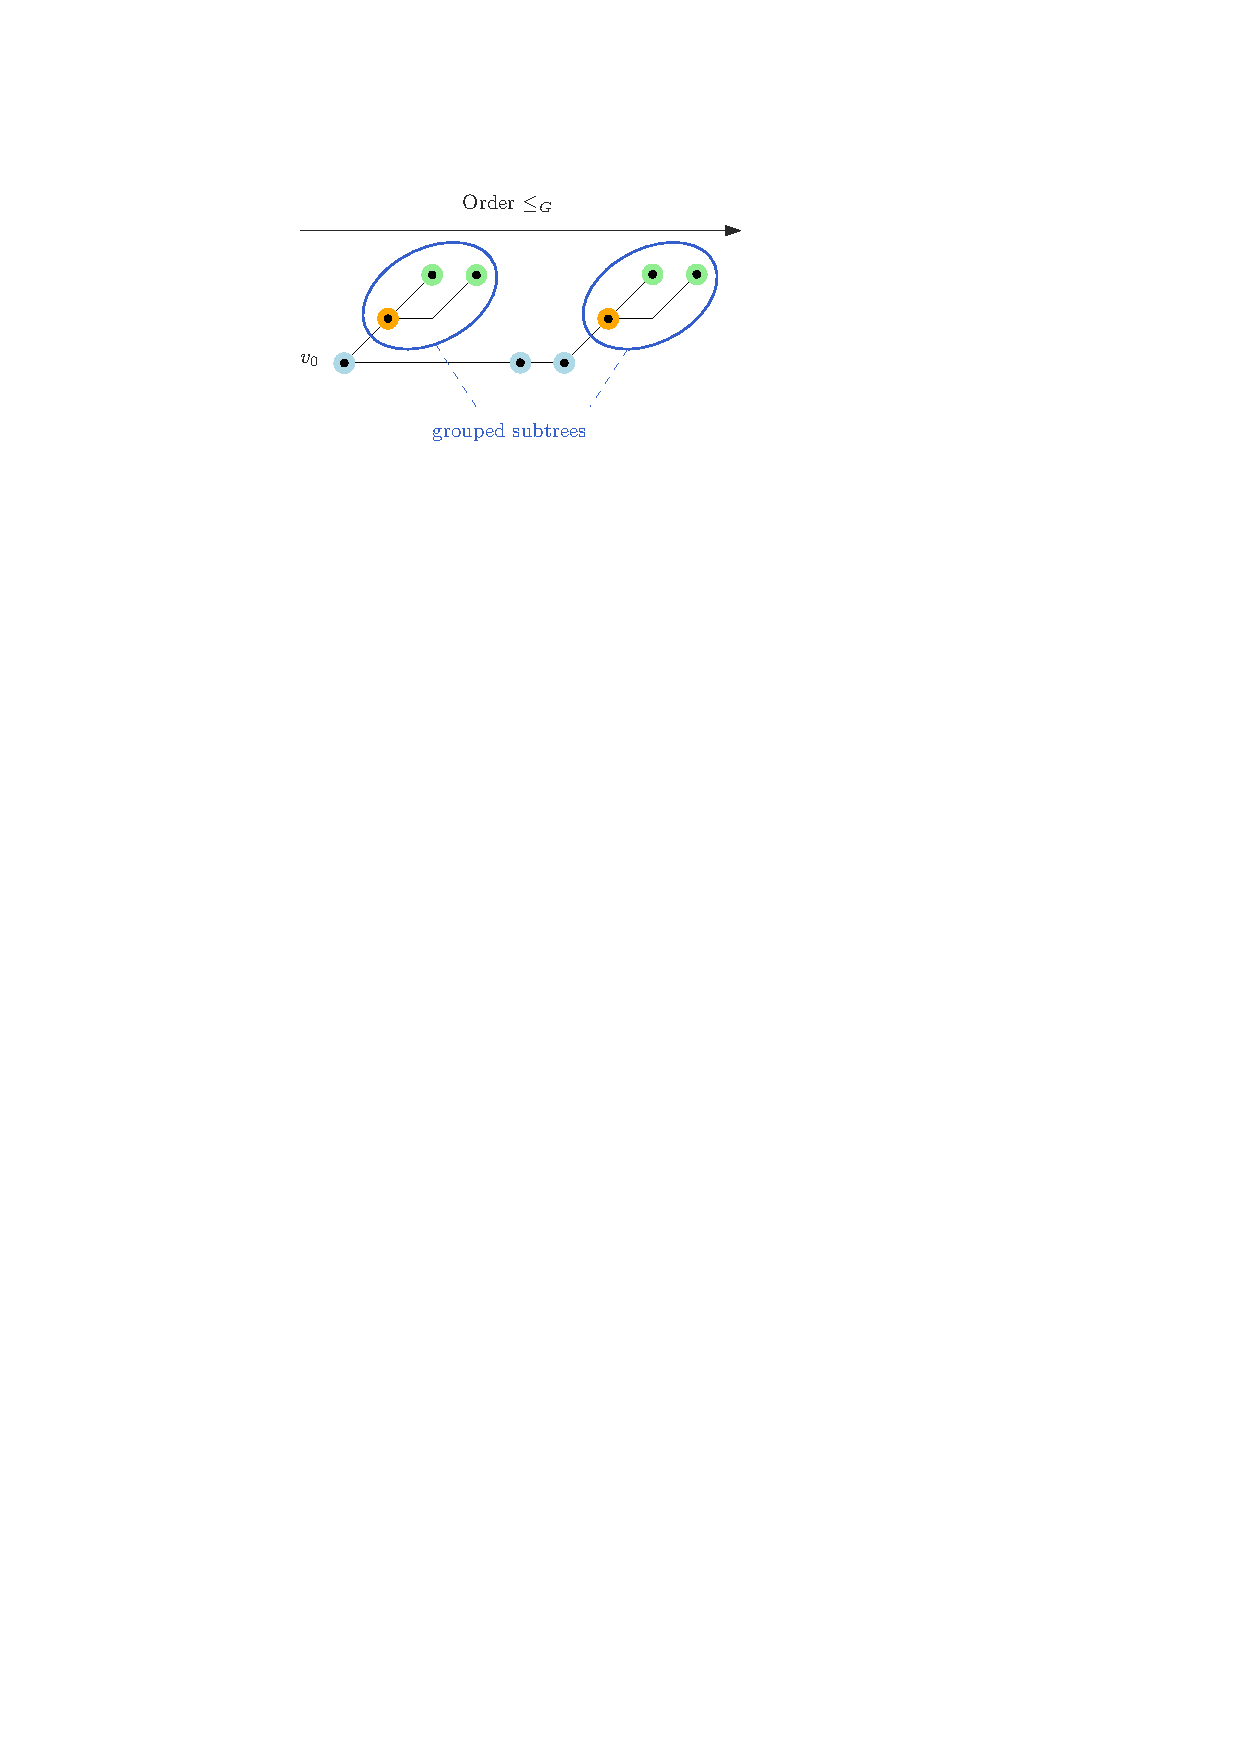
\includegraphics{graphics/ch4_order.pdf}
    \caption{An admissible order over $V$, from left to right.}
    \label{fig:ch4-order}
\end{figure}
\soeren{Make sure, you do not scale any figures in Latex. Instead, create them at the right size in ipe and import them without scaling. Makes figures more uniform among each other and with the text. It helps that the standard canvas size in ipe is A4}\peter{done, except for tikzpictures in standalone (for results plots), see 6\_evaluation.tex. What about those?}

Figure~\ref{fig:ch4-order} shows a possible embed order $\order$, which adheres to these criteria.

For a given lobster, there may be multiple possible admissible orders. Whichever one we choose, the dynamic program requires that its definition remains constant during the execution of the algorithm over all partial problem instances.

The \emph{depth} $\depth$ of a partial problem is the number of embedded vertices, i.e. the minimum $d$ vertices under $\order$. It takes $d$ subdivisions from the initial partial problem to arrive at a (set of) depth $\depth$ problems.

Let $V = V_d \cup V_r$ be a bipartition of $V$ ordered under an order $\order$, where the \emph{prefix} $V_d$ contains the smaller vertices until some cutoff vertex and $V_r$ contains the remaining larger vertices: $$\forall v_d \in V_d, v_r \in V_r: v_d \order v_r.$$ We call $V_d$ the set of ``embedded'' vertices, meaning that we have, before fully defining the totality of the embedding function $d: V \mapsto \mathbb R^2$, already decided on some $d(v)$ for every $v \in V_d$. $V_r$ are then the remaining vertices yet to be embedded. For a partial problem with depth $\depth$, $|V_d| = \depth.$

The \emph{spine head} $\coord_s$ is the coordinate of the last embedded spine vertex and the \emph{branch head} $\coord_b$ is the coordinate of the last embedded branch vertex. At depth $\depth$, 

\begin{equation*}
\begin{aligned}
\coord_s &= \mathrm{max}_{\order}(v \in V_d \cap \Spines) \text{ and} \\
\coord_b &= \mathrm{max}_{\order}(v \in V_d \cap \Branches).
\end{aligned}
\end{equation*}

Let $\coord$ be the tri-grid embedding coordinate of a spine vertex. The \emph{fundamental neighborhood} of a partial problem $$\Phi(\coord_s) = \left\{ \coord_s + \left(x + \frac y2, \frac{\sqrt3}2 y\right) \Big\vert |x + y| \leq 2; x, y \in \mathbb Z \right\}$$ is a region of interest for avoiding potentially conflicting assignments of coordinates to vertices in $V_r$. It defines a ``perceptive range'' inside of which the algorithm remembers the embedding coordinates of vertices in $V_d$ and are also potential embedding coordinates of vertices in $V_R$.

The \emph{fundament} $F \subseteq \Phi(\coord_s)$ is a subset of local grid locations which are unavailable due to being reserved for vertices in $V_d$.

Refer to Figure~\ref{fig:ch4_partialproblem} for an illustration of all the above concepts.

The \emph{signature} $\signature$ of a partial problem is the tuple $(\depth, \coord_s, \coord_b, F)$, specifying the depth, heads and fundament of the problem.

\begin{problem}[Partial UDC Recognition for Lobsters]
Given a Lobster $G$, an embedding order $\order$ and a signature $\signature$, does $G$ admit a partial tri-grid x-monotone embedding of the remaining vertices under the constraints defined by $\signature$?
\label{prob:partial-udc-lobster}
\end{problem}
\soeren[inline]{There's too much undefined notation here. Maybe you can add a definition beforehand and introduce the partial solution. The tuple $(d, \order, \coord_s, \coord_b, F)$ is often called the signature of a partial solution. You can first define all the parts, then introduce then define the signature of a partial solution.}
\peter[inline]{Better now? All parts are defined before the problem and the ``intermediate state'' is now called a signature.}

\soeren[inline]{State that the dynamic program creates partial representations for subgraphs of the input graph. the subgraphs are a prefix of length $i$ in a given admissible order, then define the admissible order. Further we need the concept of a fundamental neighborhood. Then define that. Every partial representation of a prefix is characterized by a \emph{signature}, which is a 4-tuple $(d, \gamma, \gamma, F)$ (define here what these four are). Then finally state the partial UDC recognition problem (with set of signatures).}\peter[inline]{This structure is now in place.}

\begin{figure}
    \centering
    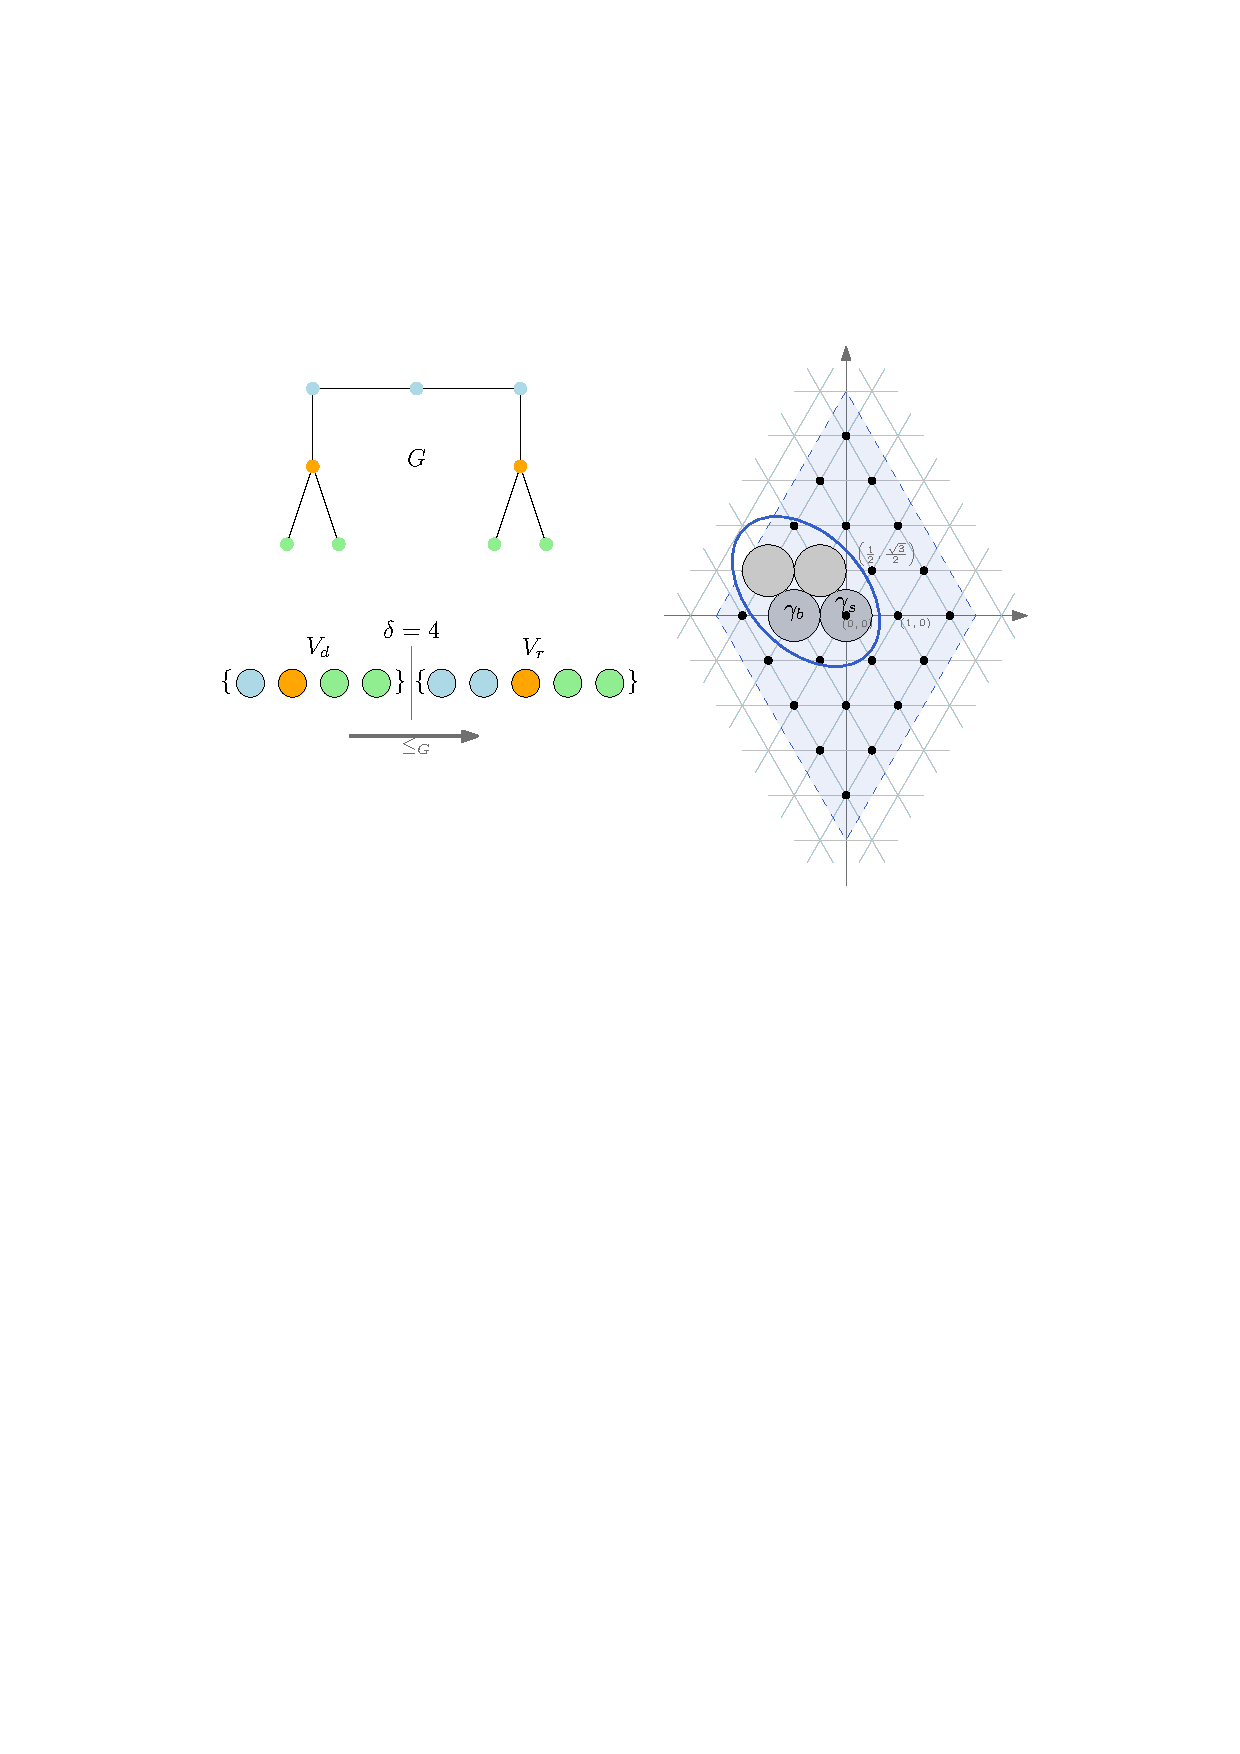
\includegraphics{graphics/ch4_partialproblem.pdf}
    \caption{An instance of Problem~\ref{prob:partial-udc-lobster}. The task is to decide the lobster depicted in the top left as a node-link diagram. Its vertices, illustrated as disks in the bottom left, are partitioned into the prefix $V_d$ and the remainder $V_r$, with the second spine vertex to be embedded next.
    On the right side, the fundamental neighborhood $\Phi(\coord_s)$ is marked with dots on the coordinates and enclosed with a dashed line. The coordinates contained in the fundament $F$ are represented by grey disks, marked with the blue band. These locations are earmarked for the embedding of the vertices in $V_d$ and no longer available for any vertices in $V_r$.}
    \label{fig:ch4_partialproblem}
\end{figure}

Figure~\ref{fig:ch4_partialproblem} visualizes a partial problem instance.

We are now prepared to define the dynamic programming algorithm on the extended problem definition.

\begin{algorithm}
\SetKwFunction{Divide}{divide}
\SetKwFunction{Sort}{sort}
\SetKwData{V}{V}
\SetKwData{Sigs}{S}
\SetKwData{sig}{$\signature$}
\SetKwData{parent}{parent}
\SetKwData{undef}{undef}
\SetKwData{Fundament}{F}
\KwIn{lobster $G = (V, E), V = \Spines \cup \Branches \cup \Leaves$}
\KwOut{``yes'' if $G$ admits a tri-grid x-monotone embedding, ``no'' otherwise}
\KwData{Set of signatures $\Sigs_\depth$ at depth $\depth$}
$n \gets |V|$\;
\V $\gets \Sort(V)$ \tcp*{establish some admissible order $\order$}
$\Sigs_0 \gets \{ \text{initial signature: } (\depth=0, \coord_s=\undef, \coord_b=\undef, \Fundament = \emptyset) \}$\;
\For{$\depth = 1$ \KwTo $n$}{
    $\Sigs_\depth \gets \bigcup\limits_{\sig \in \Sigs_{\depth-1}}$ \Divide{$\V, \sig$}\;
}
\If{$\Sigs_n = \emptyset$}{
    \Return{``no''}\;
}
\Else{
    \Return{``yes''}\;
}
\caption{The simplified dynamic program. This scheme does not implement the run-time efficiency improvements discussed later in this chapter, but it serves to illustrate the dynamic programming formula and the reasoning behind its linear-time complexity.}
\label{alg:simple-dynprog}
\end{algorithm}

For any partial problem instance $\probinst$ at the maximum depth $\depth = |V|$, there are no further vertices to embed and the answer is always ``yes'' (the input lobster does admit a tri-grid x-monotone embedding). At depth $\depth < |V|$, the answer is ``yes'' if there exists a sub-problem yes-instance of $\probinst$, and ``no'' only if no descendant instance reaches the maximum depth. We therefore subdivide partial problems until we find a maximum-depth instance or until the search space is exhausted. The algorithm will be defined such that the combined assignments of coordinates during division of the instance define a total embedding function $d(G)$.

Algorithm~\ref{alg:simple-dynprog} shows an illustrative implementation. Unlike this pseudo-code, note that the common conception of a dynamic program involves a ``combination'' of solved sub-problems into a solution of the super-problem. Because of the above conditions on ``yes''- and ``no''-instances, we can short-circuit the recombination step. See Subsection~\ref{section:ch3_earlyexit} below.

\begin{algorithm}
\SetKwFunction{Divide}{divide}
\SetKwData{Candidates}{K}
\SetKwData{Candidate}{$\kappa$}
\SetKwArray{V}{V}
\SetKwData{Sigs}{S}
\SetKwData{sig}{$\signature$}
\SetKwData{parent}{parent}
\SetKwData{undef}{undef}
\SetKwData{Fundament}{F}
\SetKwProg{Fn}{Function}{}{}
\Fn{\Divide{$\V, \signature$}}{
\KwIn{ordered vertices $\V = \Spines \cup \Branches \cup \Leaves$, signature $\signature = (\depth, \coord_s, \coord_b, \Fundament)$}
\KwOut{Set of signatures $\Sigs'$}
\KwData{Set of candidate coordinates \Candidates}

$v \gets \V{$\depth$}$\;

\If(\tcp*[f]{first vertex $\implies v \in \Spines$}){$\depth = 0$}{
    $\coord_s' \gets (0, 0)$\;
    $\Fundament' \gets \{ \coord_s' \}$\;
    \Return{$\{ (1, \coord_s', \undef, \Fundament') \}$}\;
}

$\Sigs' \gets \emptyset$\;

\If(\tcp*[f]{spine vertex}){$v \in \Spines$}{
    $\Candidates \gets \Gamma^{x+}(\coord_s) \setminus F$\;
    \ForEach{$\kappa \in \Candidates$}{
        $\Fundament' \gets (\Fundament \cap \Phi(\kappa)) \cup \{ \kappa \}$\;
        $\signature \gets (\depth+1, \kappa, \undef, \Fundament')$\;
        $\Sigs' \gets \Sigs' \cup \{ \signature \}$\;
    }
}
\ElseIf(\tcp*[f]{branch}){$v \in \Branches$}{
    $\Candidates \gets \Gamma(\coord_s) \setminus F$\;
    \ForEach{$\kappa \in \Candidates$}{
        $\Fundament' \gets \Fundament \cup \{ \kappa \}$\;
        $\signature \gets (\depth+1, \coord_s, \kappa, \Fundament')$\;
        $\Sigs' \gets \Sigs' \cup \{ \signature \}$\;
    }
}
\Else(\tcp*[f]{leaf})
{
    $\Candidates \gets \Gamma(\coord_b) \setminus F$\;
    \ForEach{$\kappa \in \Candidates$}{
        $\Fundament' \gets \Fundament \cup \{ \kappa \}$\;
        $\signature \gets (\depth+1, \coord_s, \coord_b, \Fundament')$\;
        $\Sigs' \gets \Sigs' \cup \{ \signature \}$\;
    }
}

\Return{$\Sigs'$}\;

}
\caption{Subdivision of partial problem instances. We deal with partial problems in terms of their signatures, which contain the distinguishing properties of the instance.
Dividing an instance consists of assigning the next vertex in order to one of the \emph{candidate coordinates} in \DataSty{K} relative to the appropriate (spine- or branch-) head. Each possibility becomes a sub-instance. We maintain the fundament \DataSty{F} and the heads $\coord_s$ and $\coord_b$ as appropriate, depending on the type of assigned vertex.
Recall that $\Gamma(\coord)$ and $\Gamma^{x+}(\coord)$ define the tri-grid (x-monotone) neighborhood of $\coord$.}
\label{alg:divide}
\end{algorithm}
\soeren{Maybe I have overlooked something here, but what are $\Gamma'$ and $\Gamma^{x+}$?}\peter{Added a reminder in the figure caption.}

Algorithm~\ref{alg:divide} describes the subroutine by which descendant partial problems are derived. It returns $n \leq 5$ partial embedding sub-instances (with the negligible sole exception of $\depth = 1$).
\soeren[inline]{Is the process of division already explained here? I don't think so. Maybe we should reorder some things here.}\peter[inline]{The algorithm is now pseudo-coded instead of itemized, does this help?}

\begin{figure}
    \centering
    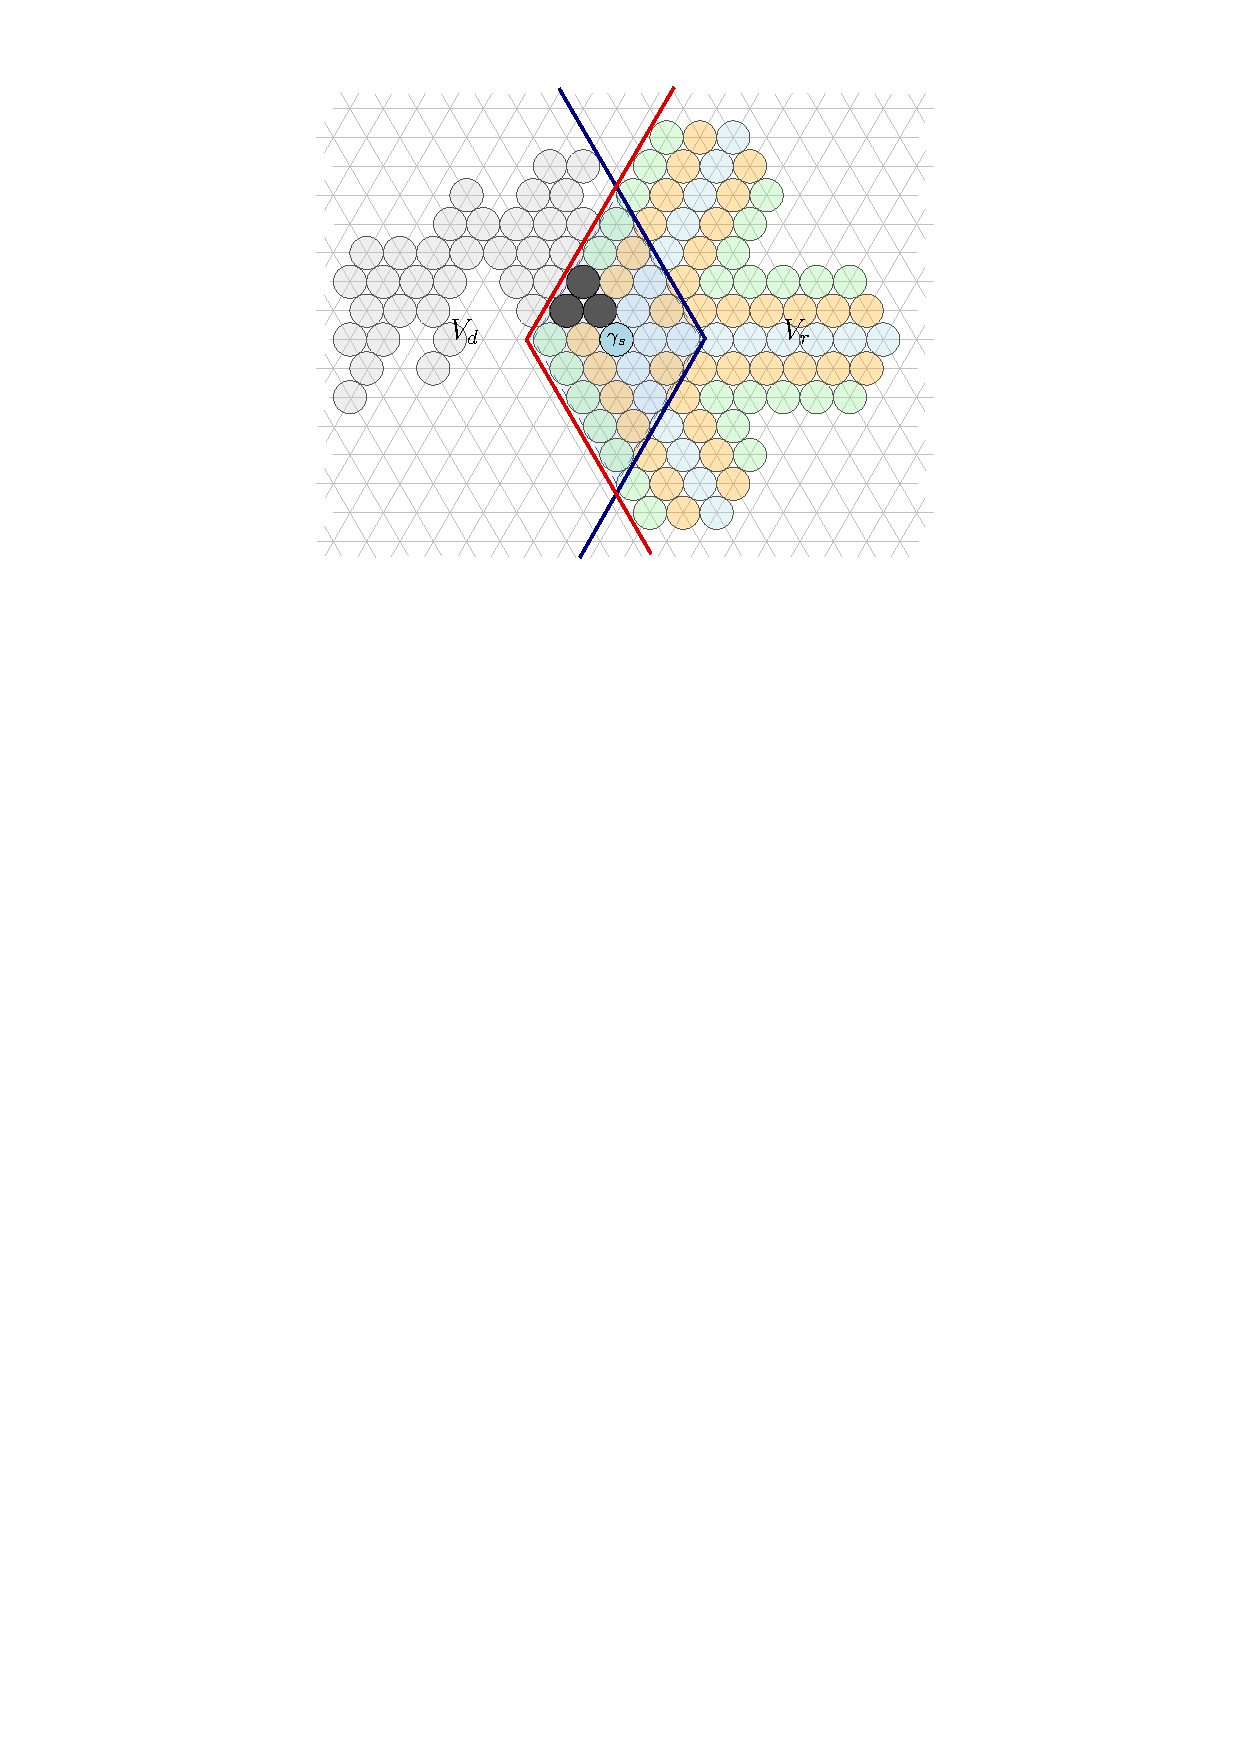
\includegraphics{graphics/ch4_reach.pdf}
    \caption{Motivation for the fundament $F$. We can imagine vertices from $V_d$ embedded in parent problems, illustrated here in translucent grey. Future $V_r$ coordinates may lie anywhere to the right, with some exemplary coordinates shown for the spine laid out only upwards, downwards or straight. The possible areas for past and future vertex coordinates are delineated in blue and red respectively, and the intersection of the areas is the fundamental neighborhood $\Phi(\coord_s)$. Vertices from $V_d$ within the fundamental neighborhood form the fundament, illustrated in solid grey. We must keep track of them for potential conflicts in coordinate assignment.}
    \label{fig:ch4_reach}
\end{figure}

\begin{figure}
    \centering
    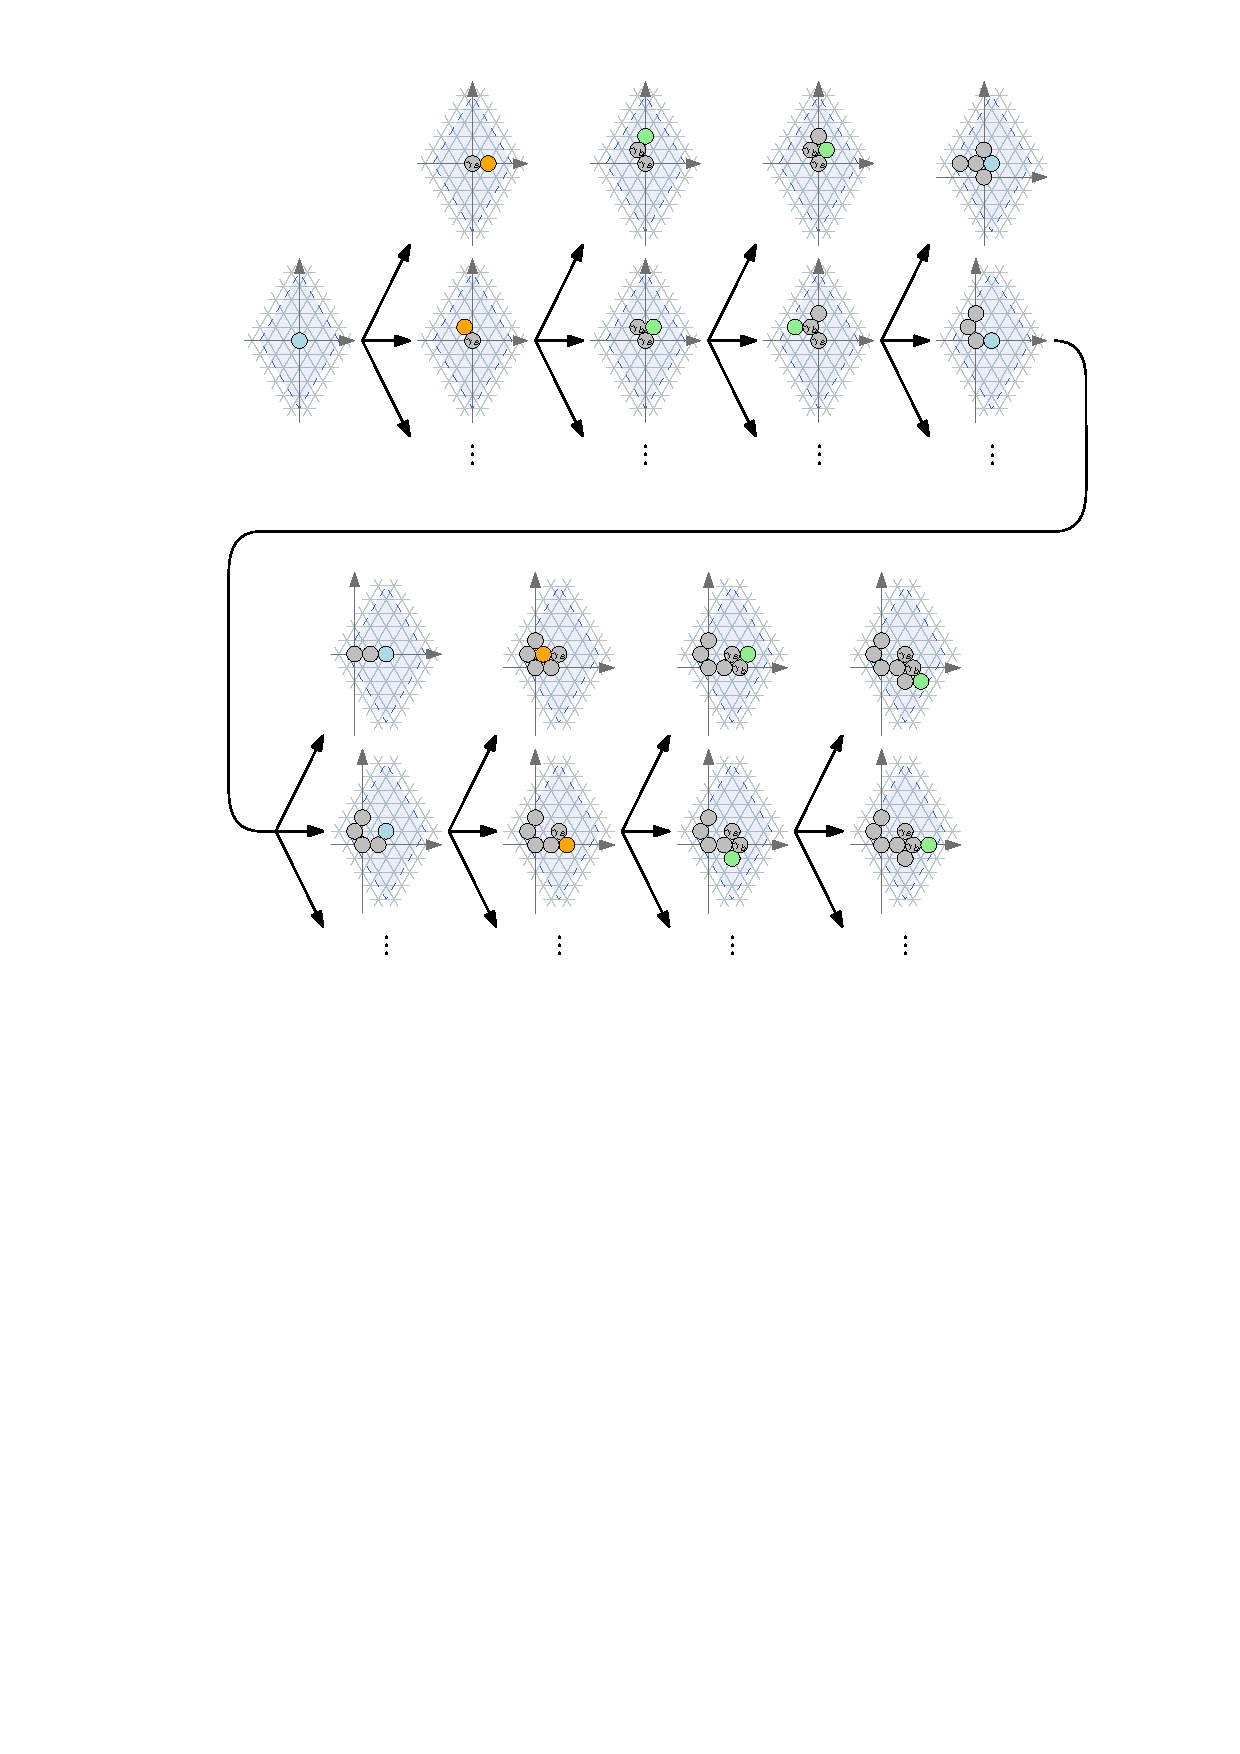
\includegraphics{graphics/ch4_dpexample.pdf}
    \caption{Example of the dynamic program approach to solve a lobster.}
    \label{fig:ch4_dpexample}
\end{figure}
\soeren{Figure~\ref{fig:ch4_dpexample} is a nice figure. But I think some transitions are not quite right.}\peter{This was the axis ``issue'' which we discussed, right? So problem solved?}

Figure~\ref{fig:ch4_dpexample} shows how the dynamic program might arrive at a decision given the same lobster as in figure~\ref{fig:ch4_partialproblem}. The arrows represent \texttt{divide} operations, yielding different paths forward. The colored disk marks the chosen candidate for the current embedding coordinate. At each point, the local knowledge of the fundament exactly suffices to prevent us from considering invalid duplicate assignments of coordinates.

\soeren[inline]{I think it will be nicer, if the two assumptions are not used as they are now, but instead after you have defined the problem and the concept of x-monotone realizations and trigrid realizations, you define a second problem, which looks specifically for such a realization.}\peter[inline]{Now properly references Problem~\ref{prob:weak-udc-lobster}, which includes the tri-grid x-monotone conditions.}

% \begin{theorem}
Given a lobster $G = (V, E)$, we can construct an initial partial UDC problem signature $\signature$ as illustrated in Algorithm~\ref{alg:simple-dynprog}.

The dynamic programming algorithm answers Problem~\ref{prob:weak-udc-lobster} on $G$.\soeren{Again clearly two different things, should be in two different Theorems. Also, If you have a Theorem, you need a proof. You can reference the original source for the proof of the base dynamic program, but your version works slightly different and maintains, different things so this still needs to be argued. We can discuss how to structure this.}\peter{Did we discuss this? Maybe an item for next meeting. :) I did remove the theorem environment for now.}
% \end{theorem}

\section{Complexity}

\begin{theorem}
Let $G = (V, E)$ be a lobster with $|V| = n$. Algorithm~\ref{alg:simple-dynprog} runs in time $O(n)$.
\end{theorem}

\begin{proof}
The determination of $\order$ and the ordered vertex set \DataSty{V} is possible in time $O(|V|)$ simply by traversing $G$ from a suitable starting spine $v_0$ of our choice (front or back).

The algorithm constructs an initial partial UDC problem signature, from which all sub-problem signatures are derived. Each problem is either \texttt{divide}d further or outright \texttt{solve}d in constant time simply by having maximum depth. Also, due to the memory of problems already encountered, no problem is processed more than once. It therefore suffices to show that the number of signatures under consideration is bound by $O(n)$.

In fact, the size of the set of signatures $\DataSty{S}_\depth$ that can be represented at any particular depth $0 \leq \depth \leq n$ is bound by a constant. Consider the constituent components of the signatures at depth $\depth$.

\begin{itemize}
    \item There is one lobster $G$ and an order $\order$ which are constant throughout the problem.
    \item The spine head $\coord_s$ does not contribute to the quantity of instances. The problem is translation-invariant. We can always derive an equivalent instance by translating $\coord_s$ to the origin point, and $\coord_b$ and $F$ with it.
    \item The branch head $\coord_b$ is relevant only when the vertex to be embedded next is a leaf, due to the subtree grouping property of $\order$. Even in that case, its position is limited to at most 6 coordinates relative to $\coord_s$.
    \item $F$ is limited to be a subset of $\Phi(\coord_s)$ and therefore to the constant amount of $2^{|\Phi(\coord_s)|} = 2^{25}$ values.
\end{itemize}
%\soeren[inline]{You could make this explicit as $n\cdot 1 \cdot 6 \cdot 2^{25} \in \mathcal{O}(n)$. Actually I am unsure if this helps the understanding.}

Since all constituent components of signatures at depth $\depth$ are limited to a constant-bound set of values and we discard duplicate signatures, the number of signatures at depth $\depth$ is also constant-bound and the total number of sub-problems is in $O(n)$. Each problem (signature) by itself takes a constant amount of time, putting the total run time in $O(n)$ as well.
\end{proof}

This result superficially seems to declare Problem~\ref{prob:weak-udc-lobster} as tractable. However, the constant bound $C$ for the number of equi-depth instances is too high to ignore for practical applications. On its face, it may be as high as

\begin{equation*}
    C = 5 \cdot 2^{24} = 83,886,080.
\end{equation*}

In this first estimate, we consider 5 locations for the branch head relative to the spine head and the spine disk before it, which eliminates one coordinate option. At depth $d>0$, $F$ always contains $\coord_s$, leaving us with just 24 potentially unavailable coordinates.

\section{Run-Time Discussion}

Consider the high constant bound $C$ of sub-problem signatures at some arbitrary depth. Upon further consideration of the algorithm definition, not every value from the domain of $\coord_b$ and $F$ can occur in real problems. Our estimate for the value of $C$ should drop accordingly. We also discuss several improvements to the algorithm which reduce the run time in practice. Some of them are based on recognizing \emph{equivalence} of signatures.

Let $\probinst_1$ with signature $\signature_1 = (\depth, \order, \coord_s^1, \coord_b^1, F^1)$ and $\probinst_2$ with signature $\signature_2 = (\depth, \order, \coord_s^2, \coord_b^2, F^2)$ be two partial recognition problem instances on the lobster $G = (V, E), |V| = n$. Let $V_r \subseteq V$ be the largest $n-\depth$ vertices under the order $\order$.

$\probinst_1$ and $\probinst_2$ are \emph{equivalent} if and only if for any witness embedding function $d_1: V_r \mapsto \R^2$ that certifies a yes-answer to $\probinst_1$, we can transform it into a yes-witness $d_2$ for $\probinst_2$ and vice-versa by translation and mirroring of the coordinates.

The global \emph{breadth} $\overline{m}$ of the graph class of lobsters is the maximum number of equivalence classes that occur at any depth over all lobsters by application of Algorithm~\ref{alg:simple-dynprog}.

\soeren[inline]{Maybe breadth should be defined in relation to a graph? Any input graph, or possible the instance of the partial embedding problem induces exactly the Breadth.}\peter[inline]{now defined for all lobsters, is this ok?}

This is important because the run time in practice is bound by $\overline{m} \cdot n$.

\subsection{Early Exit}
\label{section:ch3_earlyexit}

Our definition of the partial problem includes that the combined answer is ``yes'' iff any sub-problem answer is ``yes''. Once we find a positive instance, we can instantly skip over all other sub-problems and declare the original decision problem instance solved in the affirmative.

We encourage the fast determination of this result by always prioritizing sub-problems of higher depth before sub-problems of lower depth. We augment Algorithm~\ref{alg:simple-dynprog} with a lookup data structure of encountered (``closed'') signatures and a priority queue of pending (``open'') signatures. This allows us to customize the order of processed signatures while retaining the dynamic program benefit of not duplicating computations.

The early exit strategy does not improve the time to solve a negative instance. The algorithm is forced to check every possibility until it confirms the negative answer.

\subsection{Mirror Instance}

Let $\probinst_1$ and $\probinst_2$ be two problem instances with signatures which differ only in the branch heads $\coord_b^1$ and $\coord_b^2$ and in the fundaments $F_1$ and $F_2$. Without loss of generality, we assume that $\coord_s^1 = \coord_s^2 = (0, 0)$.

Let $m((x, y)) = (x, -y)$ be the function that mirrors coordinates along the x-axis.

$\probinst_1$ is equivalent to $\probinst_2$ if $\coord_b^1 = m(\coord_b^2)$ and $F_1 = \{m(\coord) \mid \coord \in F_2\}$.

This effectively cuts $\overline{m}$ in half.
%\soeren{Is something similar done for rotation?}\peter{No since we don't keep track of ``exhausted'' spine directions.}

\subsection{Reachability}

Define the \emph{reach} $R$ of the partial problem instance $\pi$ as the set of all possible future embedding coordinates---in other words, the disjunction of all candidate sets $K$ of all descendent sub-problem instances.

Then the unreachable coordinates $\Phi(\coord_s) \setminus R$ have no more bearing on the answer of the problem. We may as well disregard all unreachable coordinates in $\Phi(\coord_s)$ by just assuming that they are in the fundament, i.e. unavailable.

Construct the derived instance $\pi'$ equal to $\pi$, except for the fundament $F' = F \cup (\Phi(\coord_s) \setminus R)$. Then $\pi$ is equivalent to $\pi'$, and so are any other instances which differ only in the availability of unreachable coordinates.

\subsection{Domination}

Let $\probinst_1$ and $\probinst_2$ be two otherwise equal problem instances with fundaments $F_1$ and $F_2$. If $F_1 \subseteq F_2$, then $\probinst_1$ allows as many or more options for future coordinate candidates of vertices in $V_R$ than $\probinst_2$. $\probinst_1$ is easier to recognize than $\probinst_2$, and we say that $\probinst_1$ \emph{dominates} $\probinst_2$.

We can use the resulting hierarchy of instances to instantly disregard a sub-problem under consideration if, looking at the memory of known solutions, we find that we have already decided a dominating instance as a ``no''. Attempting the harder instance will never result in a ``yes''-answer.

\begin{algorithm}
\SetKw{New}{new}
\SetKw{Not}{not}
\SetKwFunction{Divide}{divide}
\SetKwFunction{Queue}{Queue}
\SetKwFunction{Priority}{priority\_predicate}
\SetKwFunction{DeMirror}{demirror}
\SetKwFunction{ApplyReachability}{apply\_reachability}
\SetKwFunction{Insert}{insert}
\SetKwFunction{Pop}{pop}
\SetKwFunction{Empty}{empty}
\SetKwFunction{ContainsDominating}{contains\_dominating}
\SetKwData{Candidates}{K}
\SetKwData{Candidate}{$\kappa$}
\SetKwData{V}{V}
\SetKwData{Sigs}{S}
\SetKwData{sig}{$\signature$}
\SetKwData{Closed}{C}
\SetKwData{parent}{parent}
\SetKwData{undef}{undef}
\SetKwData{Fundament}{F}
\SetKwProg{Fn}{Function}{}{}
\KwIn{lobster $G = (V, E), V = \Spines \cup \Branches \cup \Leaves$}
\KwOut{``yes'' if $G$ admits a tri-grid x-monotone embedding, ``no'' otherwise}
\KwData{Priority queue of open signatures \Sigs}
\KwData{Set of closed signatures \Closed}

$n \gets |V|$\;
\V $\gets$ \Sort($V$) \tcp*{establish some admissible order $\order$}
\Sigs $\gets$ \New \Queue(\Priority) \tcp*{prefer higher depth}
\Closed $\gets \emptyset$\;

\Sigs.\Insert(initial signature: $(\depth=0, \coord_s=\undef, \coord_b=\undef, \Fundament = \emptyset)$)\;

\While{$\neg$ \Sigs.\Empty()}{
    \sig $\gets$ \Sigs.\Pop()\;
    \If{\sig.$\depth$ = $n$}{
        \Return{``yes''} \tcp*{early exit}
    }
    \ForEach{\sig' $\in$ \Divide{\V, $\sig$}}{
        \ApplyReachability(\sig')\;
        \DeMirror(\sig')\;
        \If{$\neg$ \Closed.\ContainsDominating(\sig')}{
            \Sigs.\Insert(\sig')\;
            \Closed.\Insert(\sig')\;
        }
    }
}
\Return{``no''}\;
\caption{The improved dynamic program. The open queue \DataSty{S} prioritizes promising signatures, while the closed set \DataSty{C} blocks duplicates. The algorithm preprocesses signatures to combine equivalent problems.}
\label{alg:improved-dynprog}
\end{algorithm}
